\section{Target gene analysis}

As discussed in \cref{sec:circrna_mirna_sponging}, \glspl{crna} can act as
\gls{mirna} sponges and regulate the expression of target genes.
In order to investigate this regulatory mechanism, the \gls{nf-circrna}
pipeline was used to predict interactions between differentially expressed
\glspl{crna} and \glspl{mirna} that are known to be active in mouse mammary
tissue.
The dataset introduced in \cref{sec:mirna_data} was used for this analysis.
It provides a list of identified \glspl{mirna} and the target genes they are
predicted to regulate.

For each of the differentially expressed \glspl{crna}, the pipeline predicted
potential interactions with \glspl{mirna} based on sequence complementarity and
binding energy calculations.
For each \gls{crna}, the target genes of all \glspl{mirna} it interacts with
were aggregated to a single list of potential \gls{crna} target genes.
Then, gene set enrichment analysis was performed using ClusterProfiler to
identify biological processes and pathways that are significantly enriched
among the predicted target genes.

When analyzing the results, it is important to consider that the predictions
are based on the entire sequence of the \gls{crna} between the \gls{bsj} sites.
Thus, regions of the \gls{crna} that are not part of the \gls{fli} are also
considered in the analysis, which may lead to false positive predictions.

Furthermore, in contrast to the results shown in \cref{fig:esr1_go_terms}, the
target gene analysis does not provide information on the direction of
regulation.
Since all candidate \glspl{crna} are downregulated during treatment, the target
genes are expected to be upregulated.
This assumption is based on the \gls{mirna} sponge hypothesis discussed in
\cref{sec:circrna_mirna_sponging}.

The results of the target gene analysis for the differentially expressed
\glspl{crna} are shown in \cref{fig:target_genes}.

\begin{figure}[H] \begin{tabular}{ccc} \begin{subfigure}{0.5\textwidth}
                  \centering

                  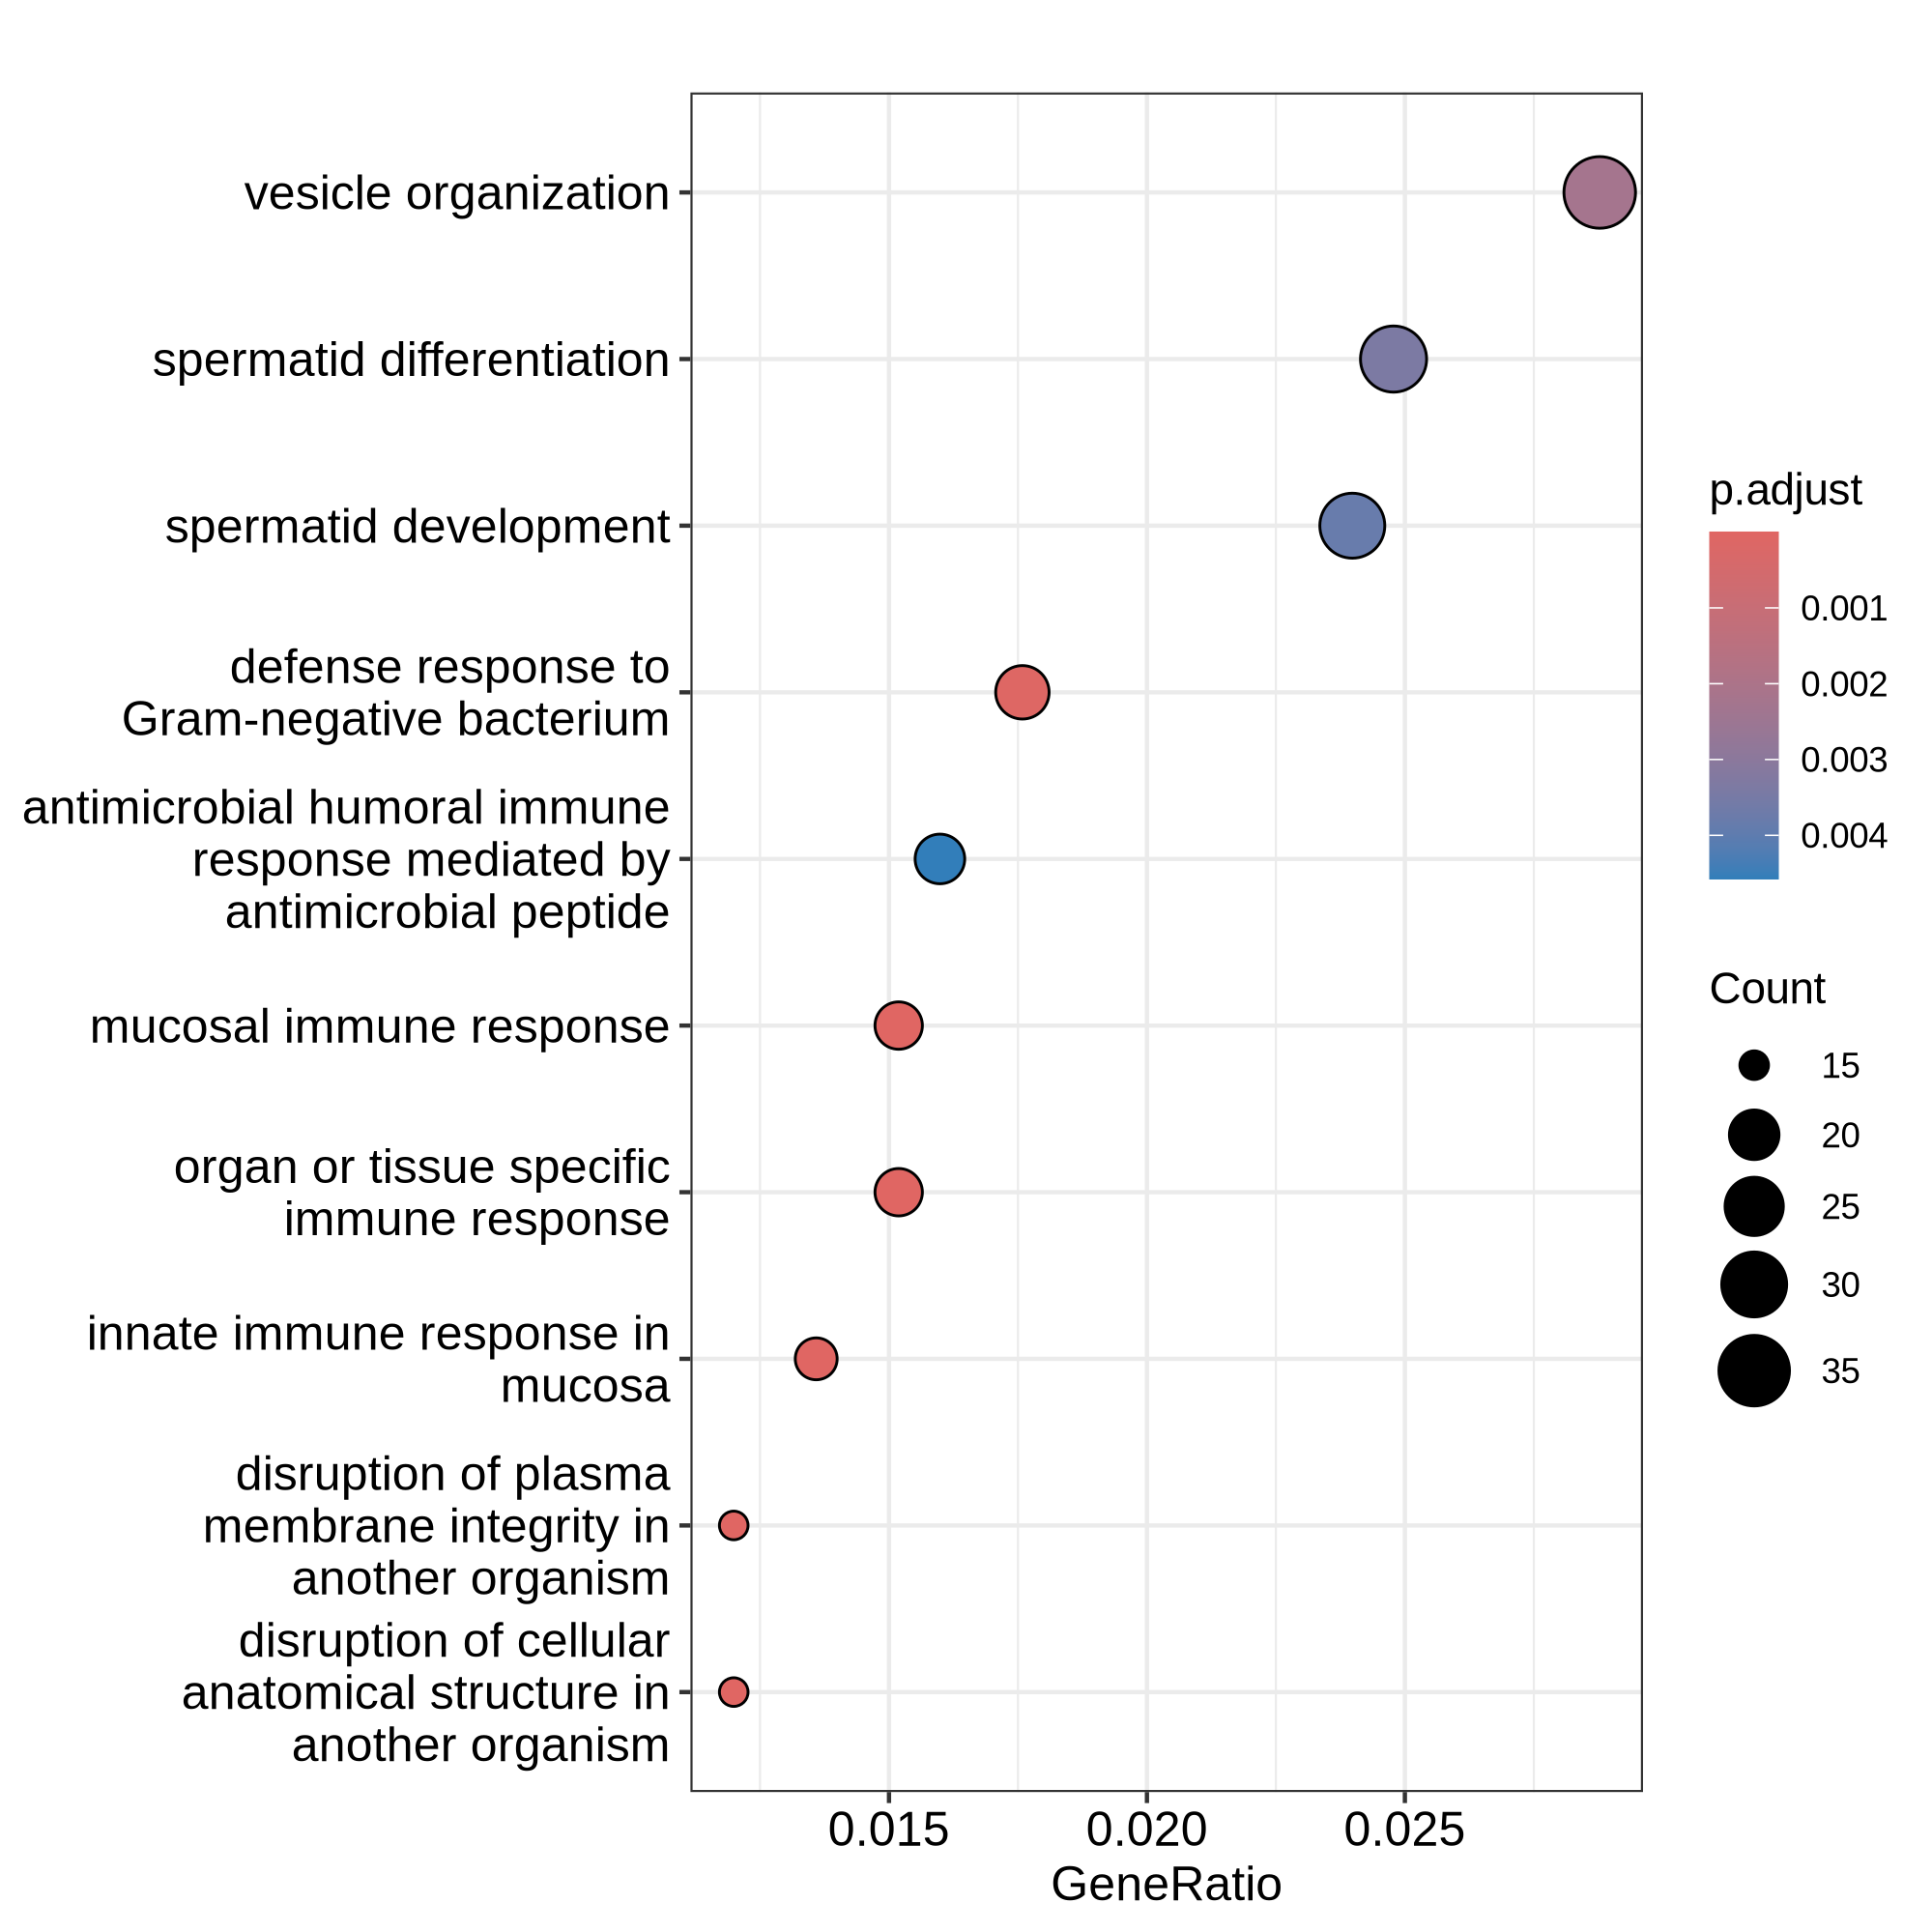
\includegraphics[width=\linewidth]{chapters/4_results_and_discussion/figures/dea/deseq2/letrozole/chr5:87925915-87926842_targets.txt.png}
                  \caption{Enriched \gls{go} terms in the target
                      genes of \textit{circ-Csn1s2a}.
                  }
                  \label{fig:tg_csn1s2a}
              \end{subfigure}
        \begin{subfigure}{0.5\textwidth}
            \centering

            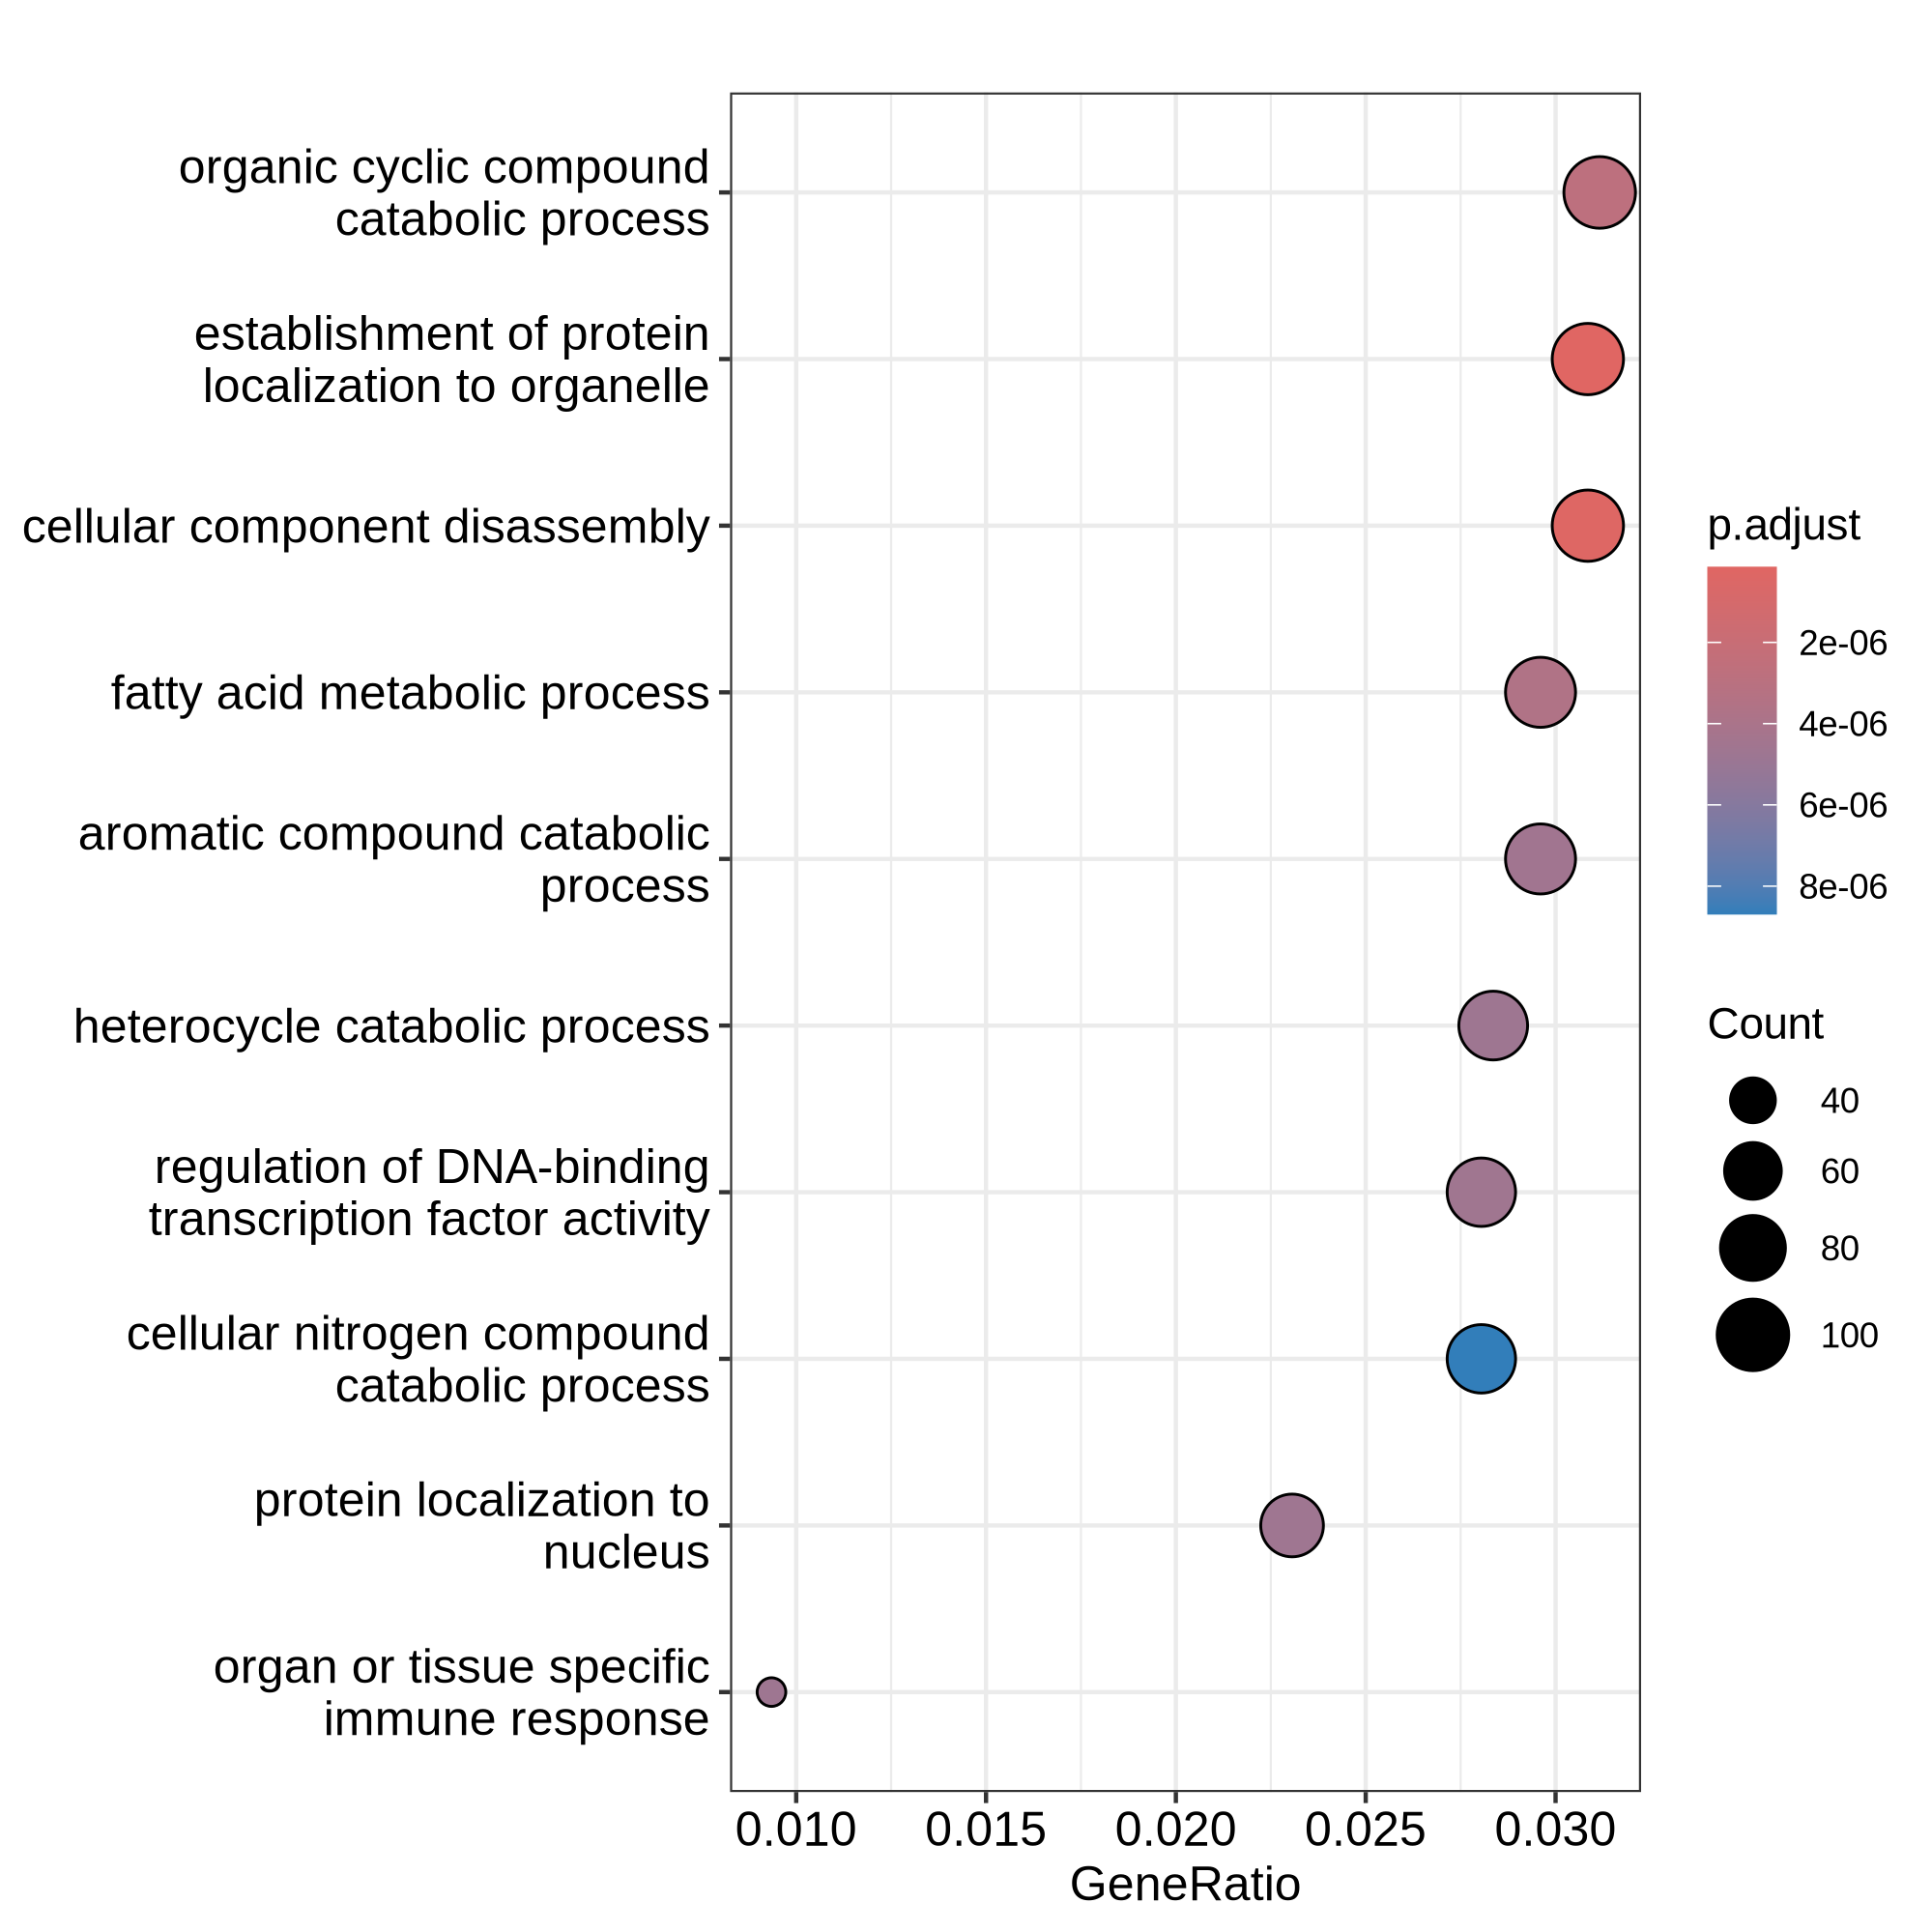
\includegraphics[width=\linewidth]{chapters/4_results_and_discussion/figures/dea/deseq2/letrozole/chr5:87817372-87821139_targets.txt.png}
            \caption{Enriched \gls{go} terms in the target
                genes of \textit{circ-Csn1s1}.
            }
            \label{fig:tg_csn1s1}
        \end{subfigure}
    \end{tabular}
    \caption{Dot plots showing the top 10 enriched terms in the predicted
        target genes of
        \textit{circ-Csn1s2a} and \textit{circ-Csn1s1}.
        \textit{Circ-Bbs9} is not shown here, as no \gls{mirna} targets were
        predicted for this \gls{crna}.
    }
    \label{fig:target_genes}
\end{figure}

While \textit{circ-Bbs9} did not have any predicted \gls{mirna} targets, the
target genes of \textit{circ-Csn1s2a} and \textit{circ-Csn1s1} showed
significant enrichment in several biological processes and pathways.

\subsection{Target genes of \textit{circ-Csn1s2a}}

As shown in \cref{fig:tg_csn1s2a}, the majority of the enriched terms in the
target genes of \textit{circ-Csn1s2} are related to immune response.
It is known that both \gls{let} and \gls{tam} interact with the immune system,
but they do so in different ways.

Tamoxifen, a \gls{serm}, has been shown to enhance the innate immune function
of neutrophils, potentially through modulation of intracellular ceramide
levels, which can affect inflammatory
responses\supercite{corriden_tamoxifen_2015}.
This suggests that tamoxifen may create a more hostile environment for tumors
by activating immune pathways.

Conversely, letrozole, an aromatase inhibitor, reduces estrogen levels, which
can also impact immune responses, particularly in the tumor microenvironment.
Studies indicate that letrozole may alter the expression of immune-associated
genes, potentially leading to different immune responses compared to tamoxifen
\supercite{dabydeen_comparison_2015}.

The tendency of \textit{circ-Csn1s2a} to high expression in untreated
samples with \gls{esr1} transgene induction and downregulation in treated
samples might suggest that \textit{circ-Csn1s2a} plays a role in suppressing
the immune response in \gls{er+} breast cancer.

\subsection{Target genes of \textit{circ-Csn1s1}}

